\documentclass[11pt]{article}

% parameters are fairly self-explanatory here, thankfully
\usepackage[width=7in,height=9.5in,top=0.75in,centering]{geometry}

% for math-ing
\usepackage{amsmath}
\usepackage{amssymb}
\usepackage{comment}

%%%%%% tables %%%%%%%%
\usepackage{tabularx}
\usepackage{array}
\renewcommand{\arraystretch}{1.5}
\setlength{\tabcolsep}{8pt}

%%%%%% plotting %%%%%%

\usepackage[dvipsnames]{xcolor}
\usepackage{tikz}
\usepackage{pgfplots}

\pgfplotsset{every axis/.append style={
                    axis x line=middle,    % put the x axis in the middle
                    axis y line=middle,    % put the y axis in the middle
                    axis line style={<->,color=black}, % arrows on the axis
                    xlabel={$x$},          % default put x on x-axis
                    ylabel={$y$},          % default put y on y-axis
            }}
            
 \pgfplotsset{compat=1.14} % sometimes, everything falls apart without this
 
 %\usepgfplotslibrary{fillbetween} %for shading between curves

%%%%%% commands %%%%%%

% exam heading; course name is first argument, exam information is second argument
\newcommand{\Heading}[2]{
    \fbox{
        {\Large\textbf{#1}}
        }
    \hfill
    \fbox{
        \begin{minipage}{0.2\textwidth}
            \begin{center}
            \textbf{#2}
            \end{center}
        \end{minipage}
    }
    \par\vspace{0.1in}}

% for being lazy while beautifying integrals
\newcommand{\dint}{\displaystyle\int}

% for being lazy while beautifying limits
\newcommand{\dlim}{\displaystyle\lim}

%%%%%% stuff %%%%%%

\usepackage{fancyhdr}

%\setcounter{page}{0} % first page is page 0

\parindent0pt % no indent

\fboxsep=0.25cm % little space in fbox border

%%%%%% BEGIN! %%%%%%%

\begin{document}

\pagestyle{fancy}

% record goals here to create sense of transparency

\fancyhead[l]{%
  \ifcase\value{page}
  % empty test for page = 0
  \or {}% 
  \or
  \or {\bf\color{ProcessBlue} F1: Lines \& Slope}% page=1
  \or {\bf\color{RoyalBlue} L1: Limits and Continuity}% page = 2
  \or {\bf\color{RoyalBlue} L2: Evaluating Limits Using Continuity and Forms}% page = 3
  \or {\bf\color{ForestGreen} D1: Meaning of a Derivative}% page = 4
  \or
  \else
  % Empty chead here!
  \fi
}

\thispagestyle{empty} % don't display that this is page 0

\Heading{MATH 1190/1210 Survey of Calculus I}{Knowledge Checkpoint 1\\Spring 2026}

\vspace{0.1in}

\textbf{Name} \hrulefill \, \begin{minipage}{0.16\textwidth}\begin{center}\textbf{UVA ID\\ (e.g. hdj4nd)} \end{center}\end{minipage}\hrulefill\\

\begin{minipage}{0.2\textwidth}\begin{center}\textbf{Course \&\\ Section Number} \end{center}\end{minipage} \hrulefill\,\,\textbf{Date} \hrulefill  \\

\hrulefill
\paragraph*{Course \& Section Numbers:}

{\small
\begin{center}
\begin{tabular}{| c | c | c | c |}
\hline
\begin{minipage}{0.12\textwidth}\centering
1190-100\\
J. Rolf\\
(2:00 PM)
\end{minipage}
&
\begin{minipage}{0.12\textwidth}\centering
1190-200\\
J. Rolf\\
(3:30 PM)
\end{minipage}
&
\begin{minipage}{0.12\textwidth}\centering
1190-100\\
Michael\\
(11 AM)
\end{minipage}
&
\begin{minipage}{0.12\textwidth}\centering
1210-200\\
Susan\\
(9:30 AM)
\end{minipage}
\\ \hline
\begin{minipage}{0.12\textwidth}\centering
1210-300\\
Susan\\
(2 PM)
\end{minipage}
&
\begin{minipage}{0.12\textwidth}\centering
1210-400\\
Holden\\
(12:30 PM)
\end{minipage}
&
\begin{minipage}{0.12\textwidth}\centering
1210-500\\
Susan\\
(3:30 PM)
\end{minipage}
&
\begin{minipage}{0.12\textwidth}\centering
1210-700\\
Aaratrick\\
(2:00 PM)
\end{minipage}
\\ \hline
\begin{minipage}{0.12\textwidth}\centering
1210-800\\
J. Bowling\\
(3:30 PM)
\end{minipage}
&
\begin{minipage}{0.12\textwidth}\centering
1210-900\\
J. Bowling\\
(5 PM)
\end{minipage}
&
\begin{minipage}{0.12\textwidth}\centering
1210-930\\
Vadim\\
(11 AM)
\end{minipage}
\\
\cline{1-3}
\end{tabular}
\end{center}
}


{%\small

\paragraph*{Instructions:}

\begin{itemize}
    
    \item The regular time allowed for completing this assessment is \fbox{$40$} minutes.
    %\item This assessment is out of 50 points.\\
    \item This assessment contains one single-part or multi-part problem for each of the following targets: {\bf\color{ProcessBlue}F1}, {\bf\color{RoyalBlue}L1}, {\bf\color{RoyalBlue}L2}, {\bf\color{ForestGreen}D1}.
    \item On each problem, you will receive a score of Exceeds Expectations (5), Proficient (4), Almost (3), Developing (2), Emerging (1), or Not Yet (0). {\bf Please do not interpret your score as a percentage.}
    %\item You will have opportunities to reassess on the targets appearing on this assessment after the next {\bf 2} assessments.\\
    \item You may NOT use calculators, dictionaries, notes, phones, or any other kind of aid.
    \item Please write neatly. What cannot be read, cannot be graded.
    \item Carefully work out each problem and clearly indicate your final answer to every problem.
    \item Throughout, give the most descriptive answer possible. \textbf{For instance, ``DNE" will not be accepted when ``$=\infty$" is applicable.}
    %\item Please provide the most specific answer possible. For instance, if a limit does not exist because it goes to $\infty$ or $-\infty$, then specify this.
    \item Please use the methods discussed up to this point in the course. For example, any work based on l'H\^opital's Rule will not receive credit.
    \item \textbf{All work must be shown unless otherwise specified.} Partial credit will not be given if appropriate work is not shown.
    \item In particular, {\bf any answer appearing with no justification will receive no credit regardless of whether the answer was correct}, unless otherwise specified.
    \item Please first respond to the prompts on which you feel most proficient, then respond to others later.
    \item This booklet is printed double-sided. It contains 8 pages and 4 numbered problems.
    \end{itemize}
    
    }

\vfill


%%%%%%%%%
\newpage

This page is left blank intentionally.\\

Use this page if you need additional space to write your solutions to any problem. \\

If you wish this page graded, you must refer to this page on \textbf{the original page} of the problem. Otherwise, your grader will NOT consider your work on this page.

\newpage%
%%%%%%%%%


\begin{enumerate}

%%%%%%%%%%%%%%%%%%%%%%%%%%%%%%%%%%%%%%%%%%%%%%%%%%%%%
%%%%%%%%%%% BEGIN PROBLEM F1 %%%%%%%%%%%%%%%%%%%%%%%%
%%%%%%%%%%%%%%%%%%%%%%%%%%%%%%%%%%%%%%%%%%%%%%%%%%%%%
\item The graph below shows the relationship between the number of hours a person has been training
and the total amount of energy consumed by the individual, measured in Calories.

\begin{center}
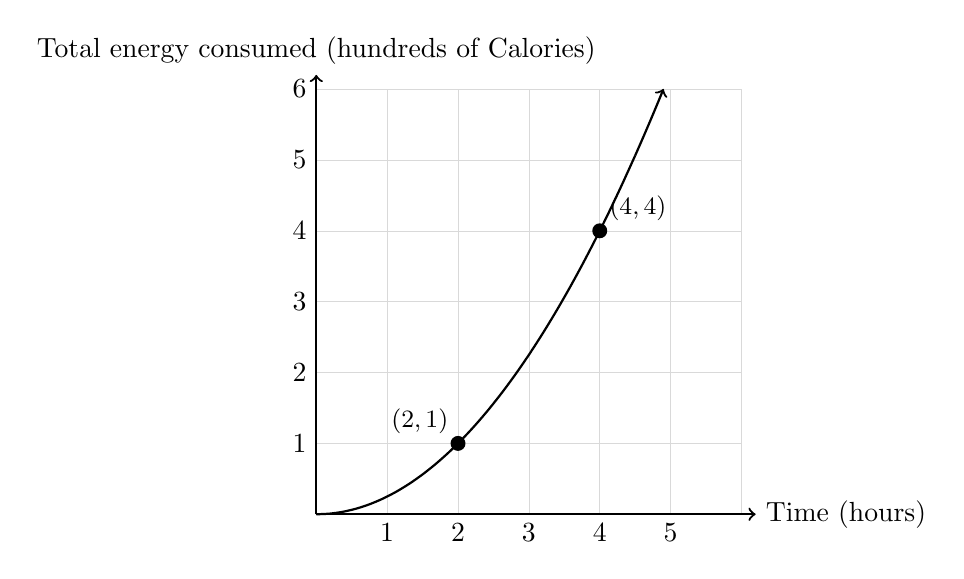
\begin{tikzpicture}[scale=0.9]

    % Grid
    \draw[step=1cm, gray!30, very thin] (0,0) grid (6,6);

    % Axes
    \draw[->, thick] (0,0) -- (6.2,0) node[right]{Time (hours)};
    \draw[->, thick] (0,0) -- (0,6.2) node[above]{Total energy consumed (hundreds of Calories)};

    % Main curve: E(t) = 0.25 t^2
    \draw[thick, smooth, domain=0:4.5]
        plot (\x, {0.25*\x*\x});

    % Arrow indicating continuation (inside grid)
    \draw[thick, ->]
        plot [domain=4.5:4.9] (\x, {0.25*\x*\x});

    % Marked integer points
 %   \fill (0,0) circle (3pt);
  %  \node[below left] at (0,0) {\small $(0,0)$};

    \fill (2,1) circle (3pt);
    \node[above left] at (2,1) {\small $(2,1)$};

    \fill (4,4) circle (3pt);
    \node[above right] at (4,4) {\small $(4,4)$};

    % Tick labels
    \foreach \x in {1,2,3,4,5}
        \node[below] at (\x,0) {\x};

    \foreach \y in {1,2,3,4,5,6}
        \node[left] at (0,\y) {\y};

\end{tikzpicture}
\end{center}



\begin{enumerate}
    \item What is the net change in energy consumed as the person goes from training for
    2 hours to 4 hours of training? Make sure to include units in your final result.

    \vfill

    \item What is the average rate of change of total energy consumed with respect to time
    over this interval? Make sure to include units in your final result.

    \vfill

    \item Use a sentence or two to explain the meaning of this average rate of change
    \textbf{in the context of this scenario}.  
    
    %Do NOT just say something vague like ``it is the average rate of change'' or ``it is the slope'' in your explanation.

    \vfill
\end{enumerate}



%%%%%%%%%%%%%%%%%%%%%%%%%%%%%%%%%%%%%%%%%%%%%%%%%%%%%
%%%%%%%%%%% END PROBLEM F1 %%%%%%%%%%%%%%%%%%%%%%%%%%
%%%%%%%%%%%%%%%%%%%%%%%%%%%%%%%%%%%%%%%%%%%%%%%%%%%%%

\newpage

%%%%%%%%%%%%%%%%%%%%%%%%%%%%%%%%%%%%%%%%%%%%%%%%%%%%%
%%%%%%%%%%% BEGIN PROBLEM L1 %%%%%%%%%%%%%%%%%%%%%%%%
%%%%%%%%%%%%%%%%%%%%%%%%%%%%%%%%%%%%%%%%%%%%%%%%%%%%%

For this problem, you may simply write your answers without showing any work.

\begin{enumerate}
    \item[(a)] Record the three continuity conditions for a function \(f(x)\) at \(x = a\):\\

    i. \rule{12cm}{0.4pt} \vspace{0.5cm} \\

    ii. \rule{12cm}{0.4pt} \vspace{0.5cm} \\

    iii. \rule{12cm}{0.4pt} \vspace{0.5cm} \\


    \item[(b)] Consider the function \(f\) graphed below. Determine the \(x\)-values, if any, at which \(f\) is discontinuous. At each number where \(f\) is discontinuous, state which condition(s) for continuity are violated.

 \noindent
\begin{minipage}[t]{0.55\textwidth}
\vspace{0pt}
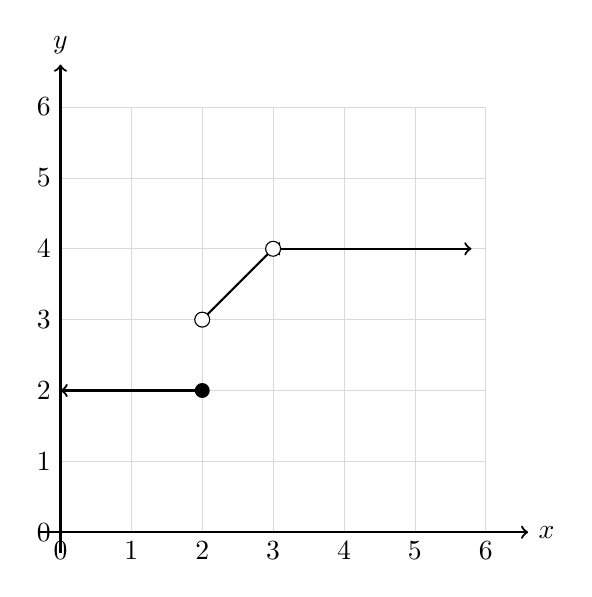
\begin{tikzpicture}[scale=0.9]
    % Grid
    \draw[step=1cm, gray!30, very thin] (0,0) grid (6,6);

    % Axes
    \draw[->, thick] (-0.3,0) -- (6.6,0) node[right]{$x$};
    \draw[->, thick] (0,-0.3) -- (0,6.6) node[above]{$y$};

    % Piecewise function with arrows
    \draw[thick, <-, domain=0:2] plot (\x, {2});
    \draw[thick, domain=2.01:2.99] plot (\x, {\x+1});
    \draw[thick, <->, domain=3:5.8] plot (\x, {4});

    % Points
    \fill (2,2) circle (3pt);
    \draw[fill=white] (2,3) circle (3pt);
    \draw[fill=white] (3,4) circle (3pt);

    % Tick labels
    \foreach \x in {0,1,2,3,4,5,6} \node[below] at (\x,0) {\x};
    \foreach \y in {0,1,2,3,4,5,6} \node[left] at (0,\y) {\y};
\end{tikzpicture}
\end{minipage}
\hspace{1em} % <-- controlled spacing instead of \hfill
\begin{minipage}[t]{0.40\textwidth}
\vspace{0pt}
\textbf{x-value:}

\vspace{3cm}

\textbf{Condition(s) violated:}

\vspace{3cm}
\end{minipage}
\vspace{5em}

    \item[(c)] Determine the types of discontinuity (if any) you found in part (b).
\end{enumerate}



%%%%%%%%%%%%%%%%%%%%%%%%%%%%%%%%%%%%%%%%%%%%%%%%%%%%%
%%%%%%%%%%% END PROBLEM L1 %%%%%%%%%%%%%%%%%%%%%%%%%%
%%%%%%%%%%%%%%%%%%%%%%%%%%%%%%%%%%%%%%%%%%%%%%%%%%%%%

\newpage

%%%%%%%%%%%%%%%%%%%%%%%%%%%%%%%%%%%%%%%%%%%%%%%%%%%%%
%%%%%%%%%%% BEGIN PROBLEM L2 %%%%%%%%%%%%%%%%%%%%%%%%
%%%%%%%%%%%%%%%%%%%%%%%%%%%%%%%%%%%%%%%%%%%%%%%%%%%%%

\item Evaluate the following limits using continuity or a specific form.

If you use continuity to evaluate a limit, to receive full credit, please provide sufficient explanation for why continuity can be used, including why the given function is continuous at the given point.

If you use a form to evaluate a limit, to receive full credit, please list the form and show all steps. 
\vspace{5em}

\begin{enumerate}
    % 1. Continuous at the point
    \item 
    \begin{tabularx}{\textwidth}{lX X}
        $\displaystyle \lim_{x\to 1} \frac{x^2 + 2x - 3}{x+1}$ & 
        \textbf{Value:} \hrulefill & 
        \textbf{Form:} \hrulefill
    \end{tabularx}
    
    \vspace{15em}


    % 2. Hierarchy / finite value
    \item 
    \begin{tabularx}{\textwidth}{lX X}
        $\displaystyle \lim_{x\to \infty} \frac{5x^2 + 3x}{2x^2 + 7}$ & 
        \textbf{Value:} \hrulefill & 
        \textbf{Form:} \hrulefill
    \end{tabularx}
    
    \vspace{15em}

    % 3. Limit goes to -∞
    \item 
    \begin{tabularx}{\textwidth}{lX X}
        $\displaystyle \lim_{x\to \infty} \frac{-3e^x - x}{\ln(x) + 5}$ & 
        \textbf{Value:} \hrulefill & 
        \textbf{Form:} \hrulefill
    \end{tabularx}

\end{enumerate}



%%%%%%%%%%%%%%%%%%%%%%%%%%%%%%%%%%%%%%%%%%%%%%%%%%%%%
%%%%%%%%%%% END PROBLEM L2 %%%%%%%%%%%%%%%%%%%%%%%%%%
%%%%%%%%%%%%%%%%%%%%%%%%%%%%%%%%%%%%%%%%%%%%%%%%%%%%%

\newpage

%%%%%%%%%%%%%%%%%%%%%%%%%%%%%%%%%%%%%%%%%%%%%%%%%%%%%
%%%%%%%%%%% BEGIN PROBLEM D1 %%%%%%%%%%%%%%%%%%%%%%%%
%%%%%%%%%%%%%%%%%%%%%%%%%%%%%%%%%%%%%%%%%%%%%%%%%%%%%
\item The figure below shows the power output, $P(I)$ (in kilowatts), of a solar panel as a function of sunlight intensity $I$ (in kW/m$^2$).

\begin{center}
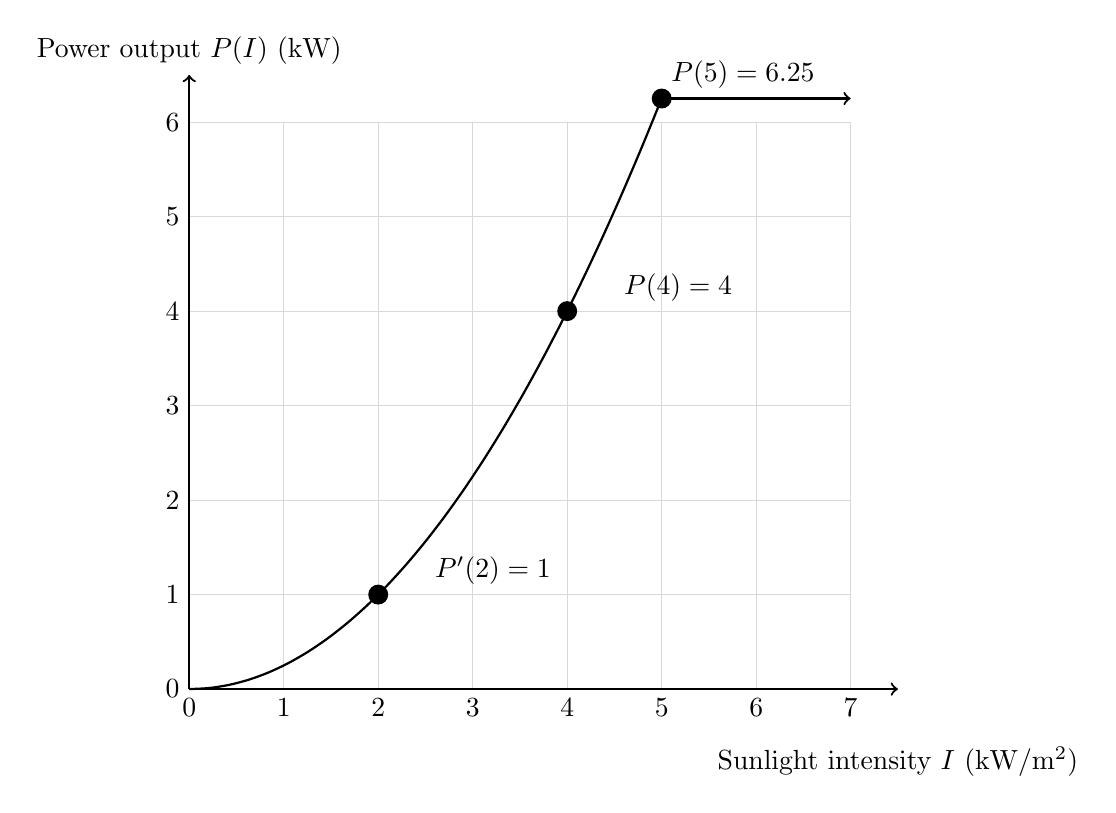
\begin{tikzpicture}[scale=1.2]
    % Grid
    \draw[step=1cm, gray!30, very thin] (0,0) grid (7,6);

    % Axes
    \draw[->, thick] (0,0) -- (7.5,0) node[below, yshift=-6mm]{Sunlight intensity $I$ (kW/m$^2$)};
    \draw[->, thick] (0,0) -- (0,6.5) node[above]{Power output $P(I)$ (kW)};

    % Concave-up parabola for 0 <= x <= 5: P(I) = 0.25*I^2
    \draw[thick, smooth, domain=0:5] plot (\x, {0.25*\x*\x});

    % Constant portion for x > 5
    \draw[thick, ->] (5,6.25) -- (7,6.25); % arrow indicating continues

    % Marked points
    %\fill (0,0) circle (3pt);
   % \node[below left, xshift=-2mm, yshift=-2mm] at (0,0) {$P(0)=0$};

    \fill (2,1) circle (3pt);
    \node[above right,xshift=6mm] at (2,1) {$P'(2)=1$};

    \fill (4,4) circle (3pt);
    \node[above right,xshift=6mm] at (4,4) {$P(4)=4$};

    \fill (5,6.25) circle (3pt);
    \node[above right] at (5,6.25) {$P(5)=6.25$};

    % Tick labels
    \foreach \x in {0,1,2,3,4,5,6,7} \node[below] at (\x,0) {\x};
    \foreach \y in {0,1,2,3,4,5,6} \node[left] at (0,\y) {\y};

\end{tikzpicture}
\end{center}




\begin{enumerate}
    \item Use a sentence or two to explain the meaning of the equation $P(4)=4$ in this context. 

    To receive full credit, please include units for all quantities discussed, and write your answer \textbf{in the context of the problem}.

    \vfill 

    \item Use a sentence or two to explain the meaning of the equation $P'(2)=1$ in this context. 

    To receive full credit, please include units for all quantities discussed, and write your answer \textbf{in the context of the problem}.
        \vfill

    \item What is the value of $P'(5)$? To receive full credit, explain why.

    \vfill
\end{enumerate}




%%%%%%%%%%%%%%%%%%%%%%%%%%%%%%%%%%%%%%%%%%%%%%%%%%%%%
%%%%%%%%%%% END PROBLEM D1 %%%%%%%%%%%%%%%%%%%%%%%%%%
%%%%%%%%%%%%%%%%%%%%%%%%%%%%%%%%%%%%%%%%%%%%%%%%%%%%%

\newpage

This page is left blank intentionally.\\

Use this page if you need additional space to write your solutions to any problem. \\

If you wish this page graded, you must refer to this page on \textbf{the original page} of the problem. Otherwise, your grader will NOT consider your work on this page.

\newpage

This page is left blank intentionally.\\

Use this page if you need additional space to write your solutions to any problem. \\

If you wish this page graded, you must refer to this page on \textbf{the original page} of the problem. Otherwise, your grader will NOT consider your work on this page.

\end{enumerate}

\end{document}